\documentclass[12pt,a4paper]{article}
\usepackage[T2A]{fontenc}
\usepackage[utf8]{inputenc}
\usepackage[russian]{babel}
\usepackage{amsmath}
\usepackage{amssymb}
\usepackage{graphicx}
\usepackage{floatrow}
\usepackage{booktabs}
\usepackage{wrapfig}
\usepackage{lipsum}
\usepackage{subcaption}
\usepackage{fancyhdr}

\newcommand{\figref}[1]{(См. рис. \ref{#1})}
\newcommand{\secref}[1]{(См. раздел. \ref{#1})}

\newcommand{\e}[1]{\text{$\cdot10^{#1}$}}

\pagestyle{fancy}
\fancyhead{}
\fancyhead[L]{Работа 3.6.1}
\fancyhead[R]{}
\fancyfoot[C]{\thepage}

\author{\normalsize Выполнил: Голубович Тимур, группа Б01-108 \\
	\normalsize 17.09.2022}
\date{}

\usepackage{float}
\restylefloat{table}
\title{
	\large Отчет о выполнении лабораторной работы 3.6.1 \\
	\Large Спектральный анализ электрических сигналов \\ 
	
}


\begin{document}
\maketitle
	
\section*{Цель работы}
Изучить спектральный состав периодических электрических сигналов.

\section*{Оборудование и приборы} 
Компьютер  с \emph{PicoScope 6}; \newline
функциональный генератор \emph{waveStation 2052}; \newline
USB-осциллограф \emph{АКИП-4108}.
	
	
\section*{Теоретическое введение}

Рассмотрим функцию вида 
\begin{equation}\label{f}
	f(x) = \sum_{n=1}^{N}A_n \cos(\omega_n t -\alpha_n),
\end{equation}
где $ A_n, \omega_n, \alpha_n $ -- постоянные величины. Множество пар $ (\omega_i, A_i) $ называется спектром $ f(x) $ и может быть конечным или бесконечным.

Периодический сигнал может быть представлен в виде ряда Фурье:

\begin{equation}\label{key}
	f(t) = \frac{a_0}{2}+\sum_{n=1}^{\infty}(A_n \cos(n \Omega_1 t - \psi_n)),
\end{equation}

где $ a_0/2 = const $ -- среднее значение функции, $ A_n $ -- амплитуды членов разложения. Спектр любой периодической функции можно представить в виде набора гармонических колебаний с дискретными частотами $ \Omega_1 = \frac{1}{T_1}, 2\Omega_1, \ldots $ и постоянной составляющей с нулевой частотой. Такой спектр называется линейчатым или дискретным.

Непериодический сигнал представим в виде интеграла Фурье. В данной работе исследование таких сигналов не проводится.

Для периодического прямоугольного сигнала $ \left< V \right> = V_0 \frac{\tau}{T} $, $ A_n \sim \frac{\sin x}{x} $. Здесь и далее шириной спектра $ \Delta \nu $ называем расстояние от главного максимума до 1-го нуля огибающей. При этом выполнено соотношение неопределённостей:

\begin{equation}\label{eq:неопр}
	\Delta \nu \tau \simeq 1
\end{equation}

\begin{figure}[h]
	\begin{minipage}{0.49\linewidth}
		\centering
		\includegraphics[width=0.9\linewidth]{"res/square"}
		\label{fig:spectr}
	\end{minipage}
	\begin{minipage}{0.49\linewidth}
		\centering
		\includegraphics[width=0.9\linewidth]{"res/spectre_square"}
	\end{minipage}
	\caption{Периодический прямоугольный сигнал}
	\label{fig:sq}
\end{figure}

Для последовательности цугов с длительностью $ \tau  $ и периодом $ T $ разложение в спектр представлено на рисунке \ref{fig:zug}.

\begin{figure}[h]
	\begin{minipage}{0.49\linewidth}
		\centering
		\includegraphics[width=0.9\linewidth]{"res/zug"}
	\end{minipage}
	\begin{minipage}{0.49\linewidth}
		\centering
		\includegraphics[width=0.9\linewidth]{"res/spzug"}
	\end{minipage}
	\caption{Периодическая последовательность цугов}
	\label{fig:zug}
\end{figure}

В случае АМ-колебаний, сигнал определяется формулой:

\begin{equation}\label{key}
	f(t) = A_0 \left(1+m \cos \Omega t \right) \cos \omega_0 t,
\end{equation}

где $ m $ -- глубина модуляции.
Спектр такого сигнала на рис. \ref{fig:AM}. Причём амплитуды синусов $ \omega_0 \pm \Omega $ равны $ m/2 $, а все начальные фазы одинаковы. То есть,

\begin{equation}
	\frac{a_\text{бок}}{a_\text{осн}} = \frac{U_{min}^S}{U_{max}^S} = \frac{m}{2}
	\label{eq:new}
\end{equation} 

Глубину модуляции можно рассчитать по формуле:

\begin{equation}
	m = \frac{A_{max}-A_{min}}{A_{max}+A_{min}}
	\label{eq:m}
\end{equation}

\begin{figure}[h]
	\begin{minipage}{0.49\linewidth}
		\centering
		\includegraphics[width=0.9\linewidth]{"res/AM"}
	\end{minipage}
	\begin{minipage}{0.49\linewidth}
		\centering
		\includegraphics[width=0.9\linewidth]{"res/spAM"}
	\end{minipage}
	\caption{АМ-сигнал}
	\label{fig:AM}
\end{figure}

При частотной модуляции мгновенная частота колебания равна:

\begin{equation}\label{m}
	\omega(t) = \omega_0+\Delta \omega_m \cdot \sin \Omega t,
\end{equation}
где $\Delta \omega = 2\pi \Delta f_m$ - амплитуда отклонения частоты (девиация частоты),
$\Omega = 2\pi F$ – модулирующая частота.

Величина $\beta = \frac{\Delta \omega_m}{\Omega} = \frac{\Delta f_m}{F}$ называется индексом частотной модуляции.


\section*{Экспериментальная установка}

Установка, используемая в работе, представлена на рис. \ref{fig:scheme}.

\begin{figure}[h]
	\centering
	\caption{Схема экспериментальной установки}
	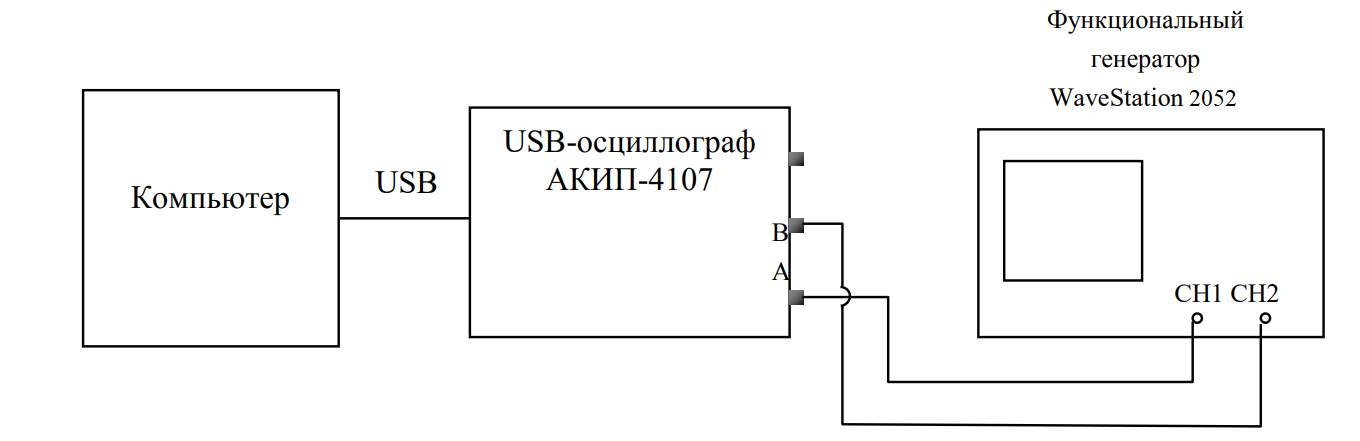
\includegraphics[width=1\linewidth]{res/scheme}
	\label{fig:scheme}
\end{figure}

Функциональный генератор позволяет сформировать два различных электрических сигнала, которые выводятся на два независимых канала USB-осциллографа.
Инструментальные погрешности считаются малыми.










\section*{Ход работы}

\subsection*{Исследование спектра периодической последовательности
прямоугольных импульсов}

Как меняется спектр сигнала ($\Delta \nu$ и $\delta \nu$) при изменении $\tau$ и фиксированной $f_\text{повт}$, а также при изменении $f_\text{повт}$ и фиксированном $\tau$ видно на рисунках \ref{fig:7a} и \ref{fig:7b}.

\begin{figure}[H]
	\centering
	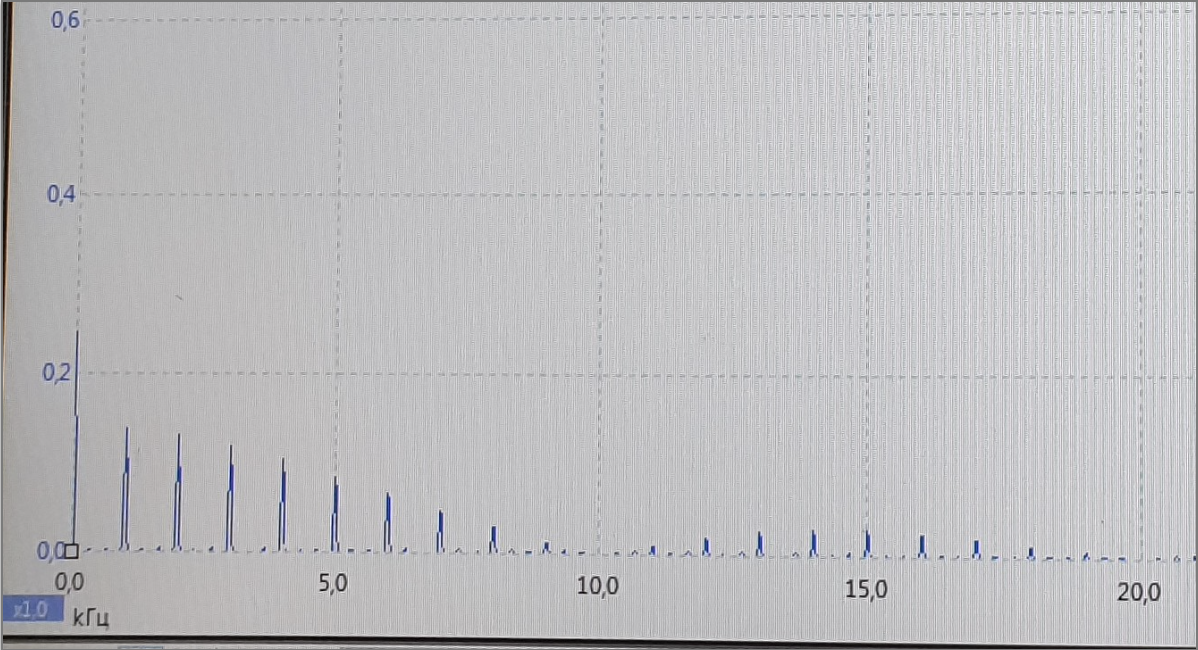
\includegraphics[width = 7 cm]{src/7_0.png}
	\caption{Спектр при $f_\text{повт} = 1 \text{ кГц}, \tau = 100 \text{ мкс}$}
\end{figure}

\begin{figure}[H]
	\centering
	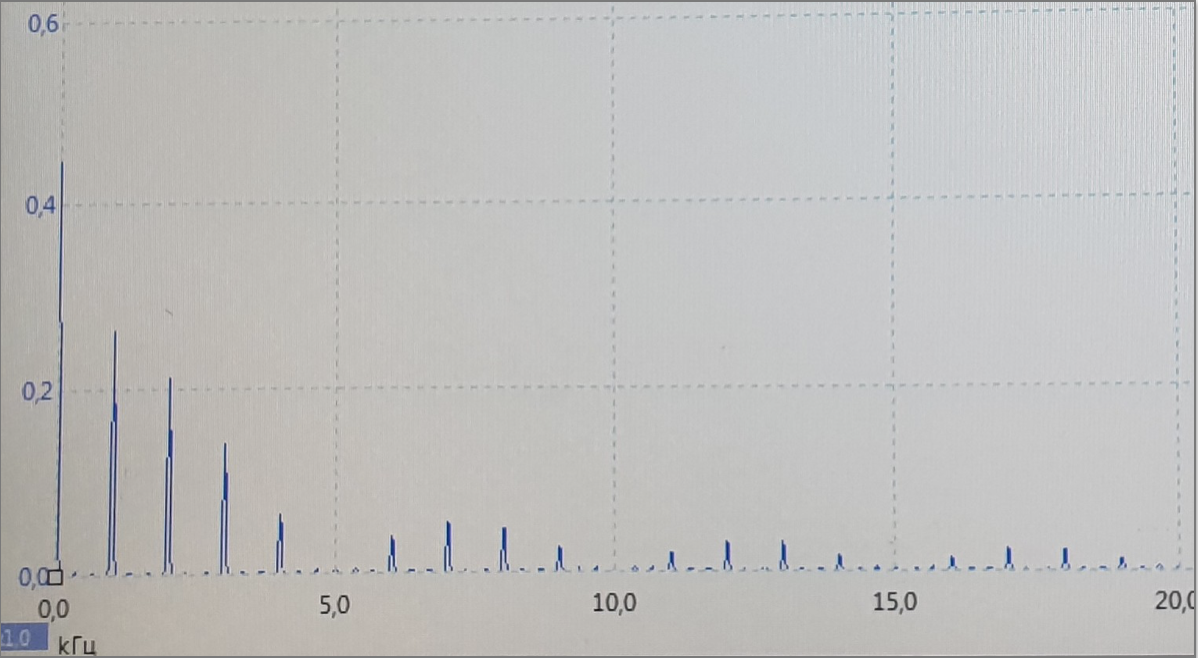
\includegraphics[width = 7 cm]{src/7_a.png}
	\caption{Спектр при $f_\text{повт} = 1 \text{ кГц}, \tau = 200 \text{ мкс}$}
	\label{fig:7a}
\end{figure}

\begin{figure}[H]
	\centering
	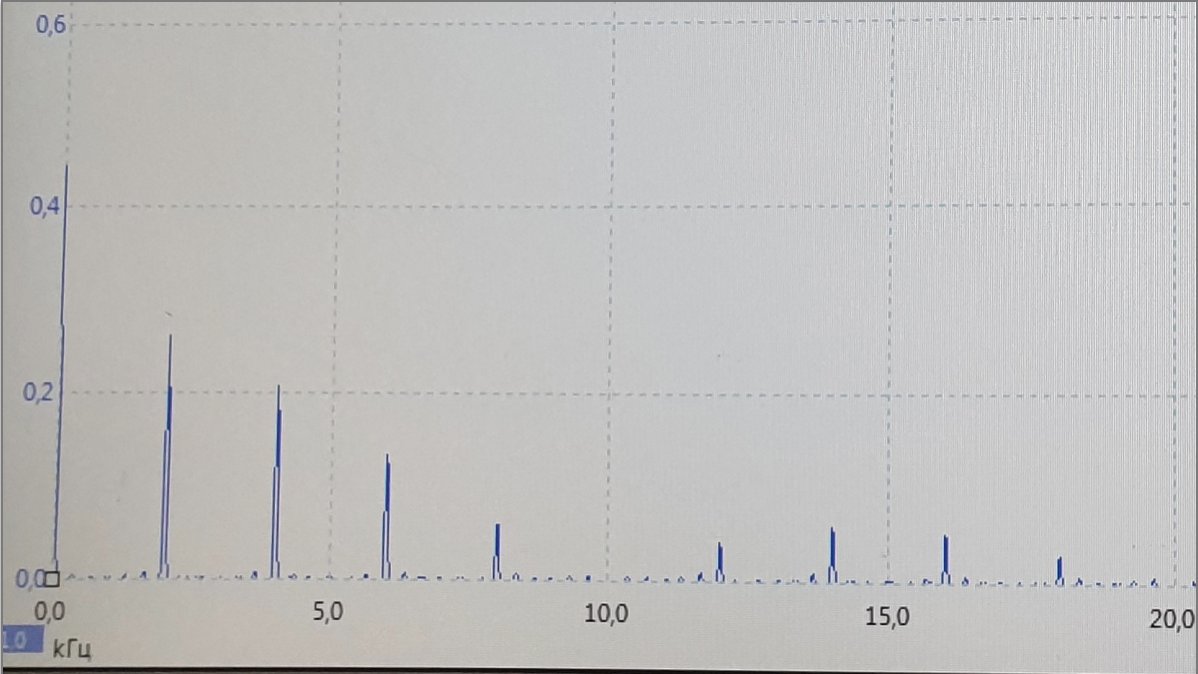
\includegraphics[width = 7 cm]{src/7_b.png}
	\caption{Спектр при $f_\text{повт} = 2 \text{ кГц}, \tau = 100 \text{ мкс}$}
	\label{fig:7b}
\end{figure}

Проведём измерения зависимости ширины спектра $\Delta \nu$ от длительности импульса $\tau$ и запишем их в таблицу \ref{tab:8}.

\begin{table}[H]
    \caption{Зависимость $\Delta \nu (\tau)$ для $f_\text{повт} = 1 \text{кГц}$}
    \begin{tabular}{ccc}
\toprule
$\tau$, мкс & $\Delta \nu$, кГц & $\frac{1}{\tau}, \text{мкс}^{-1}$\\
\midrule
40  & 25,0 & 0,0250 \\
60  & 16,0 & 0,0167 \\
80  & 13,0 & 0,0125 \\
100 & 10,0 & 0,0100 \\
120 & 8,0  & 0,0083 \\
140 & 7,0  & 0,0071 \\
160 & 6,0  & 0,0063 \\
180 & 5,5  & 0,0056 \\
200 & 5,0  & 0,0050 \\
\bottomrule
\end{tabular}
	\label{tab:8}
\end{table}

\begin{figure}[h]
	\centering
	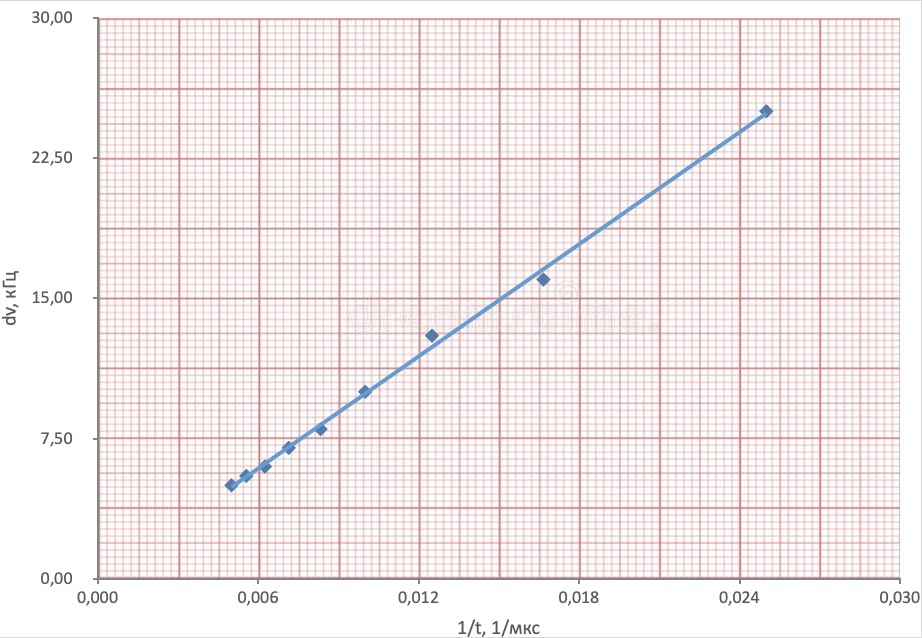
\includegraphics[width = 10 cm]{src/8.png}
	\caption{График $\Delta \nu (\tau)$}
	\label{fig:8}
\end{figure}

По графику коэффициент наклона $k = (0,999 \pm 0,05) \;\;\;\; \varepsilon_k = 5 \%$, что отлично сходится с теоретическим значением $k=1$.

Измерим частоты и амплитуды спектральных составляющих сигнала при $f_\text{повт} = 1 \text{ кГц}$ для $\tau = 50 \text{ мкс}$ и $\tau = 100 \text{ мкс}$. Запишим результаты в таблицу \ref{tab:9}.

\begin{table}[H]
    \caption{Измерения спектров для $\tau = 50 \text{ мкс}$ и $\tau = 100 \text{ мкс}$}
    \begin{table}
\begin{tabular}{ccc|ccc}
\toprule
\multicolumn{3}{c}{$\tau = 50 \text{ мкс}$} & \multicolumn{3}{c}{$\tau = 100 \text{ мкс}$} \\
$\text{№ гармоники}$ & $\nu$, кГц & $A$, мВ & $\textnumero \text{№ гармоники}$ & $\nu$, кГц & $A$, мВ\\
\midrule
0  & 0,04 & 94,10 &	0  & 0,1  & 142,70  \\
1  & 1,00 & 32,60 &	1  & 1,0  & 65,80   \\
2  & 2,04 & 33,20 &	2  & 2,0  & 62,70   \\
3  & 2,99 & 31,98 &	3  & 3,0  & 57,20   \\
4  & 3,99 & 30,14 &	4  & 4,0  & 48,59   \\
5  & 4,95 & 28,29 &	5  & 5,0  & 41,21   \\
6  & 6,03 & 27,00 &	6  & 6,0  & 33,21   \\
7  & 6,99 & 25,00 &	7  & 7,0  & 22,74   \\
8  & 7,90 & 22,00 &	8  & 8,0  & 14,15   \\
9  & 9,03 & 20,10 &	9  & 9,0  & 6,77    \\
10 & 10,00& 19,00 &	10 & 10,0 & 0,00    \\   
11 & 11,00& 17,22 &    &      &         \\
12 & 12,00& 16,60 &    &      &         \\
13 & 13,00& 14,15 &    &      &         \\
14 & 13,90& 11,67 &    &      &         \\
15 & 15,00& 9,84  &    &      &         \\
16 & 16,00& 7,38  &    &      &         \\
17 & 17,00& 5,50  &    &      &         \\
18 & 18,00& 6,15  &    &      &         \\	
\bottomrule
\end{tabular}
\end{table}

	\label{tab:9}
\end{table}

\begin{figure}[H]
	\centering
	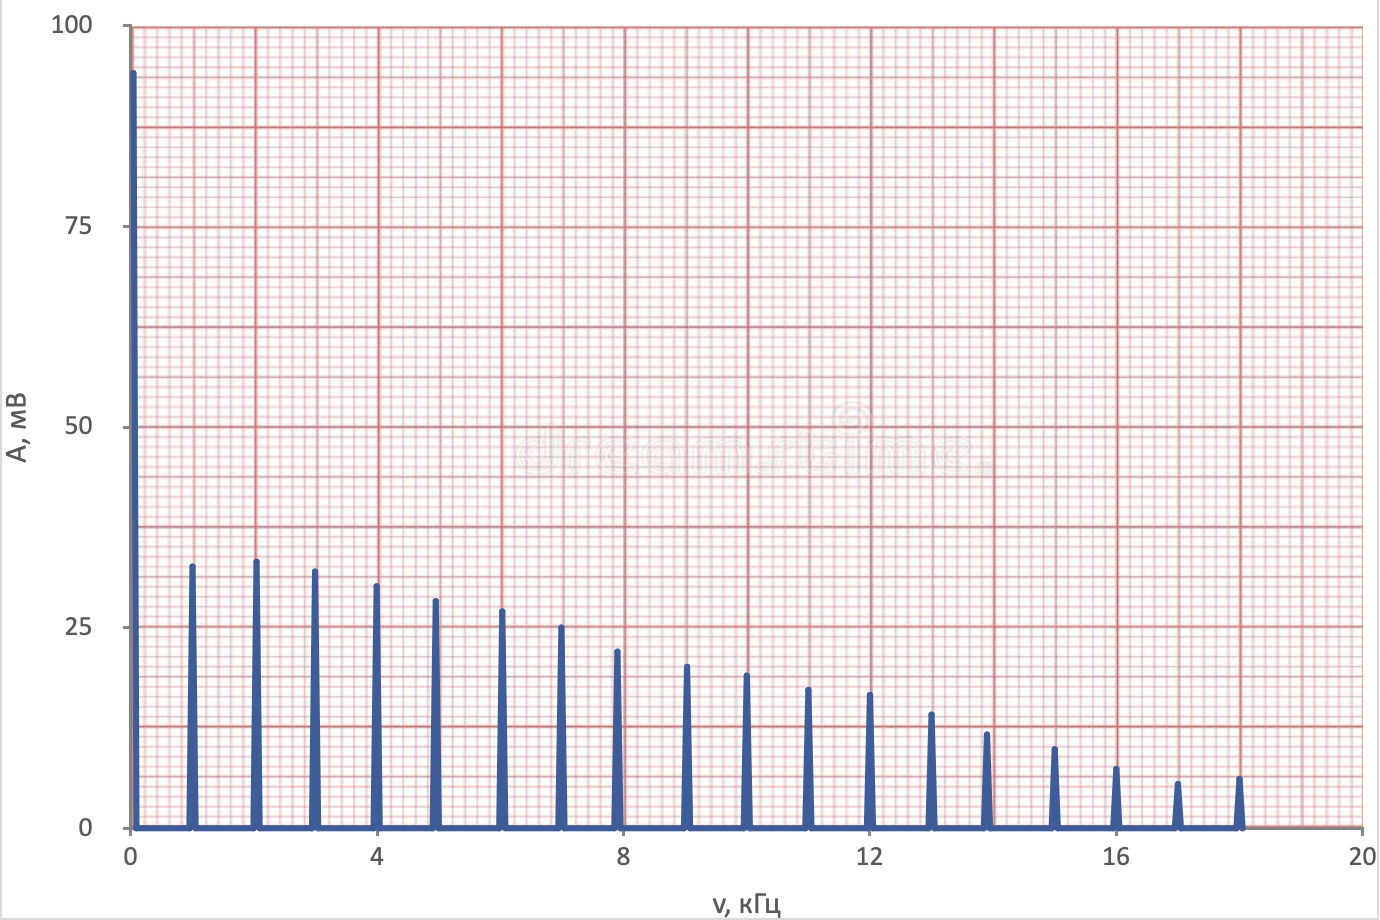
\includegraphics[width = 10 cm]{src/9_50.png}
	\caption{Спектр для $\tau = 50 \text{ мкс}$}
\end{figure}

\begin{figure}[H]
	\centering
	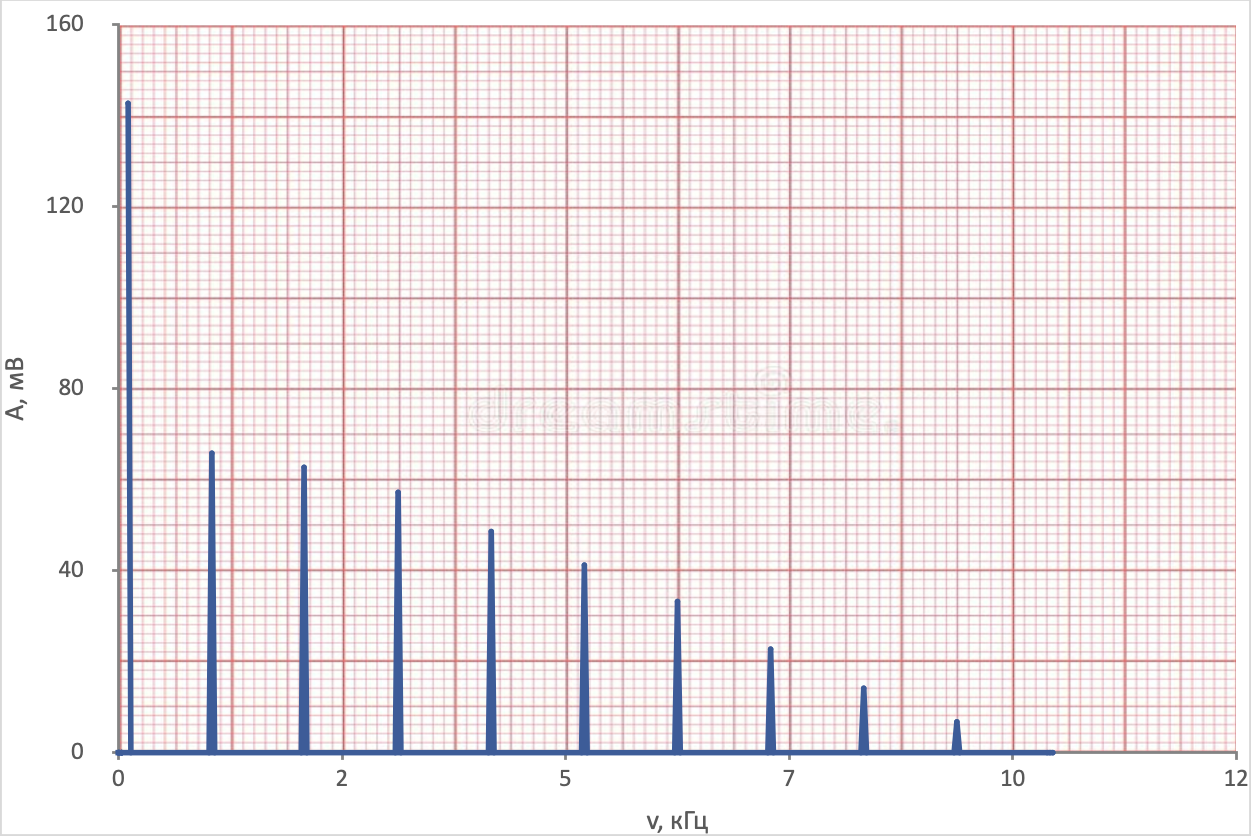
\includegraphics[width = 10 cm]{src/9_100.png}
	\caption{Спектр для $\tau = 100 \text{ мкс}$}
\end{figure}



\subsection*{Исследование спектра периодической последовательности цугов гармонических колебаний}

Посмотрим, как изменяется вид спектра при увеличении длительности $\tau$ импульса вдвое от 100 до 200 мкс.

\begin{figure}[H]
	\centering
	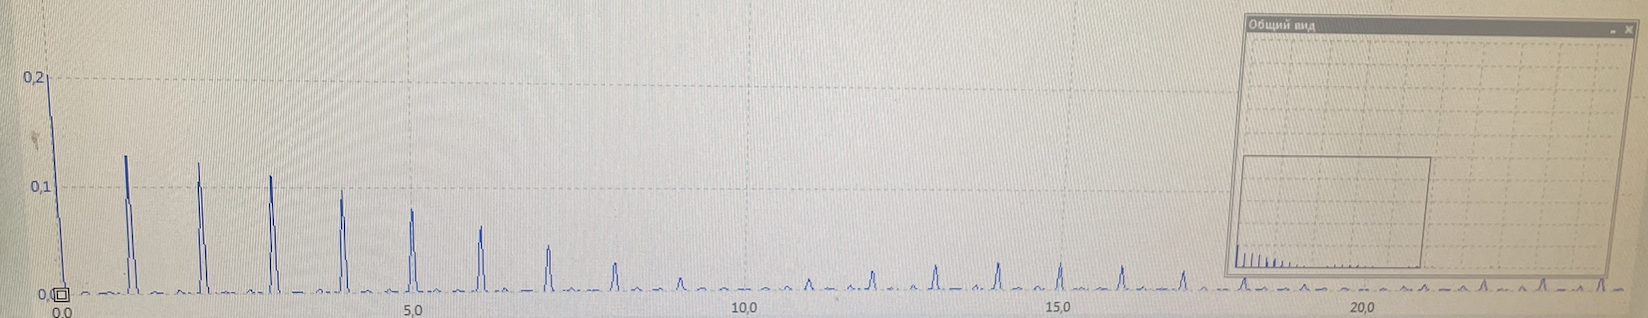
\includegraphics[width = 7 cm]{src/16a.png}
	\caption{Спектр при $\tau = 100 \text{ мкс}$}
	\label{fig:16a}
\end{figure}

\begin{figure}[H]
	\centering
	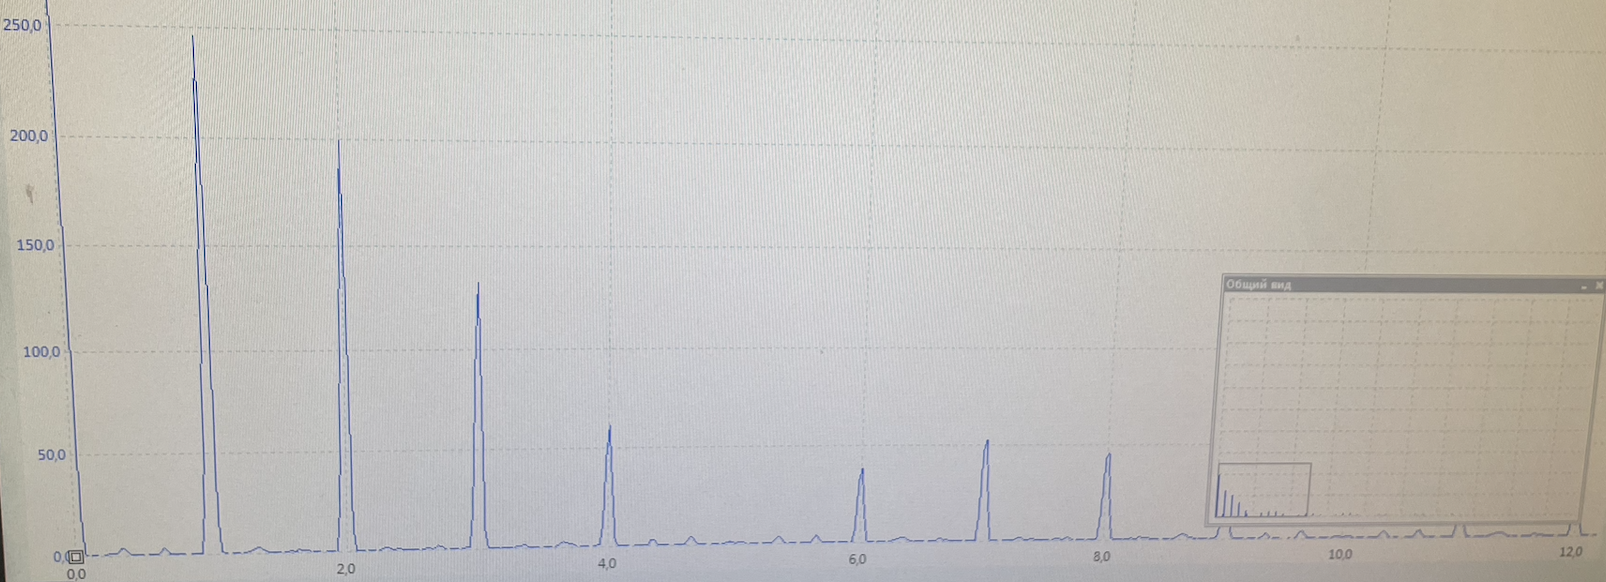
\includegraphics[width = 7 cm]{src/16b.png}
	\caption{Спектр при $\tau = 200 \text{ мкс}$}
	\label{fig:16b}
\end{figure}

Также посмотрим, как меняется картина спектра при изменении несущей частоты $\nu_0$ ($\nu_0$ = 10, 25 и 40 кГц).

\begin{figure}[H]
	\centering
	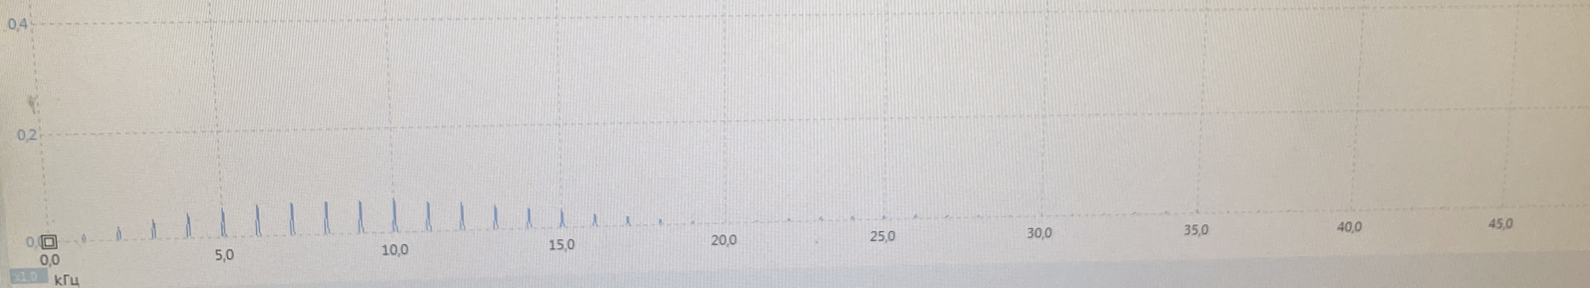
\includegraphics[width = 7 cm]{src/17_10.png}
	\caption{Спектр при $\nu_0 = 10 \text{ кГц}$}
	\label{fig:17_10}
\end{figure}

\begin{figure}[H]
	\centering
	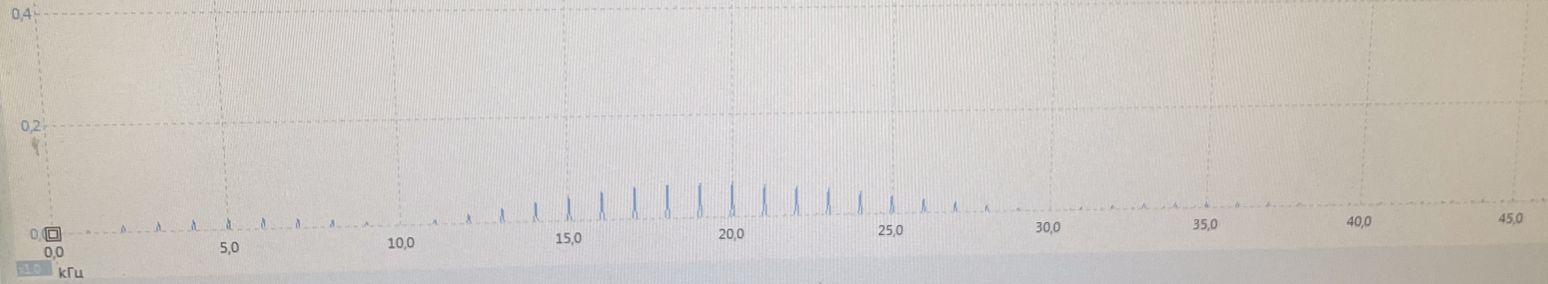
\includegraphics[width = 7 cm]{src/17_25.png}
	\caption{Спектр при $\nu_0 = 25 \text{ кГц}$}
	\label{fig:17_25}
\end{figure}

\begin{figure}[H]
	\centering
	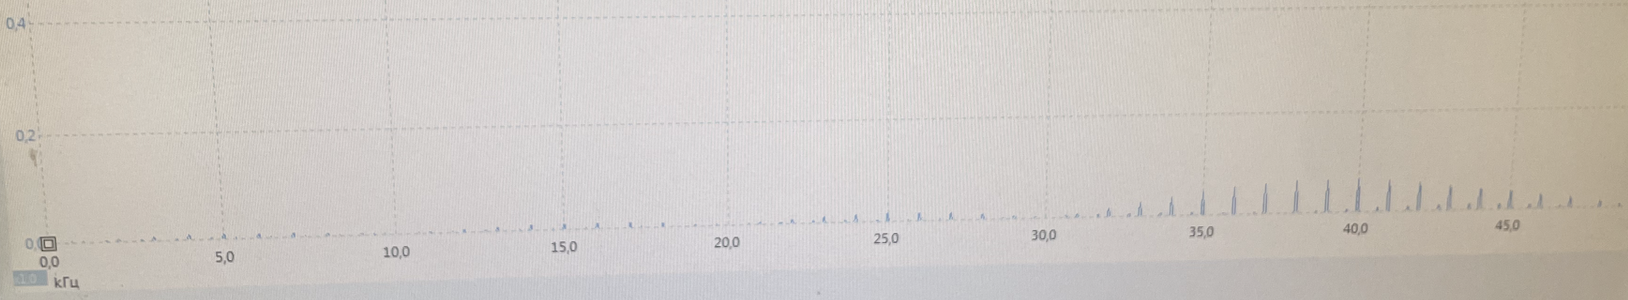
\includegraphics[width = 7 cm]{src/17_40.png}
	\caption{Спектр при $\nu_0 = 40 \text{кГц}$}
	\label{fig:17_40}
\end{figure}

Установим частоту несущей $\nu_0$ = 30 кГц, длительность импульса $\tau$ = 100 мкс. Будем определять расстояние $\delta \nu$ между соседними спектральными компонентами для разных частот повторения импульсов $f_\text{повт}$. Проведём измерения для $f_\text{повт}$ = 0,5, 1, 2, 4 и 5 кГц и запишем их в таблицу \ref{tab:18}.

\begin{table}[H]
    \caption{Зависимость $\delta \nu$ от $f_\text{повт}$}
    \begin{tabular}{cc}
\toprule
$\delta \nu$, кГц & $f_\text{повт}$, кГц \\
\midrule
0,5	& 0,5 \\
1	& 1   \\
2	& 2   \\
4	& 4   \\
5	& 5   \\
\bottomrule
\end{tabular}
	\label{tab:18}
\end{table}

\begin{figure}[H]
	\centering
	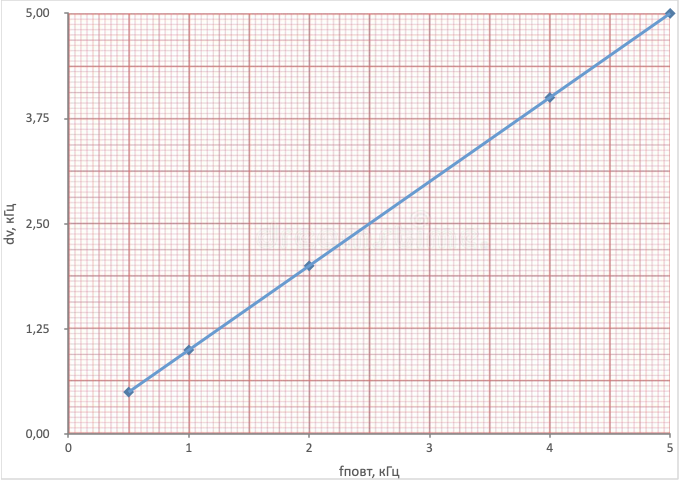
\includegraphics[width = 10 cm]{src/20.png}
	\caption{График $\delta \nu$($f_\text{повт}$)}
	\label{fig:20}
\end{figure}

Коэффициент наклона графика \ref{fig:20} 1, что опять-таки сходится с теоретическим значением.

Установим $\tau$ = 100 мкс, $f_\text{повт}$ = 1 кГц и проведём иизмерения амплитуды и частоты спектра. Результаты запишим в таблицу \ref{tab:19}. Аналогично измерения проведём для импульса с $\tau$ = 100 мкс и $f_\text{повт}$ = 2 кГц. Построим графики этих спектров.

\begin{table}[H]
    \caption{Измерения спектров для $f_\text{повт}$ = 1 кГц и $f_\text{повт}$ = 2 кГц}
    \begin{table}
\begin{tabular}{ccc|ccc}
\toprule
\multicolumn{3}{c}{$f_\text{повт}$ = 1 кГц} & \multicolumn{3}{c}{$f_\text{повт}$ = 2 кГц} \\
$\text{№ гармоники}$ & $\nu$, кГц & $A$, мВ & $\textnumero \text{№ гармоники}$ & $\nu$, кГц & $A$, мВ\\
\midrule
30 & 30 & 73 & 15 & 30 & 130 \\
31 & 31 & 55 & 31 & 32 & 105 \\
32 & 32 & 54 & 32 & 34 & 84  \\
33 & 33 & 48 & 33 & 36 & 55  \\
34 & 34 & 40 & 34 & 38 & 38  \\
35 & 35 & 33 & 35 & 40 & 24  \\
36 & 36 & 26 &    &    &     \\			
37 & 37 & 19 &    &    &     \\			
38 & 38 & 11 &    &    &     \\			
39 & 39 & 5  &    &    &     \\			
40 & 40 & 1  &    &    &     \\			
\bottomrule
\end{tabular}
\end{table}

	\label{tab:19}
\end{table}

\begin{figure}[H]
	\centering
	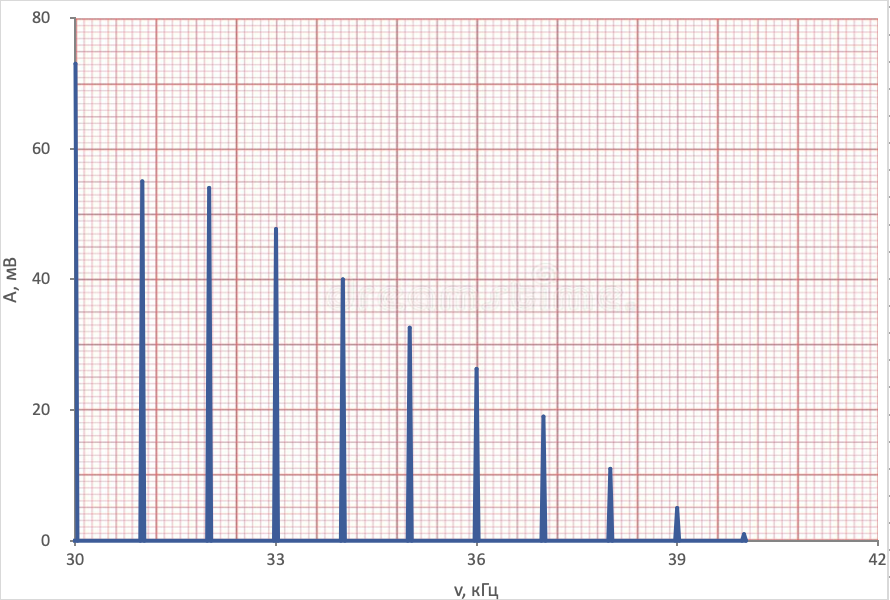
\includegraphics[width = 10 cm]{src/19_1.png}
	\caption{Спектр при $f_\text{повт}$ = 1 кГц}
	\label{fig:19_1}
\end{figure}

\begin{figure}[H]
	\centering
	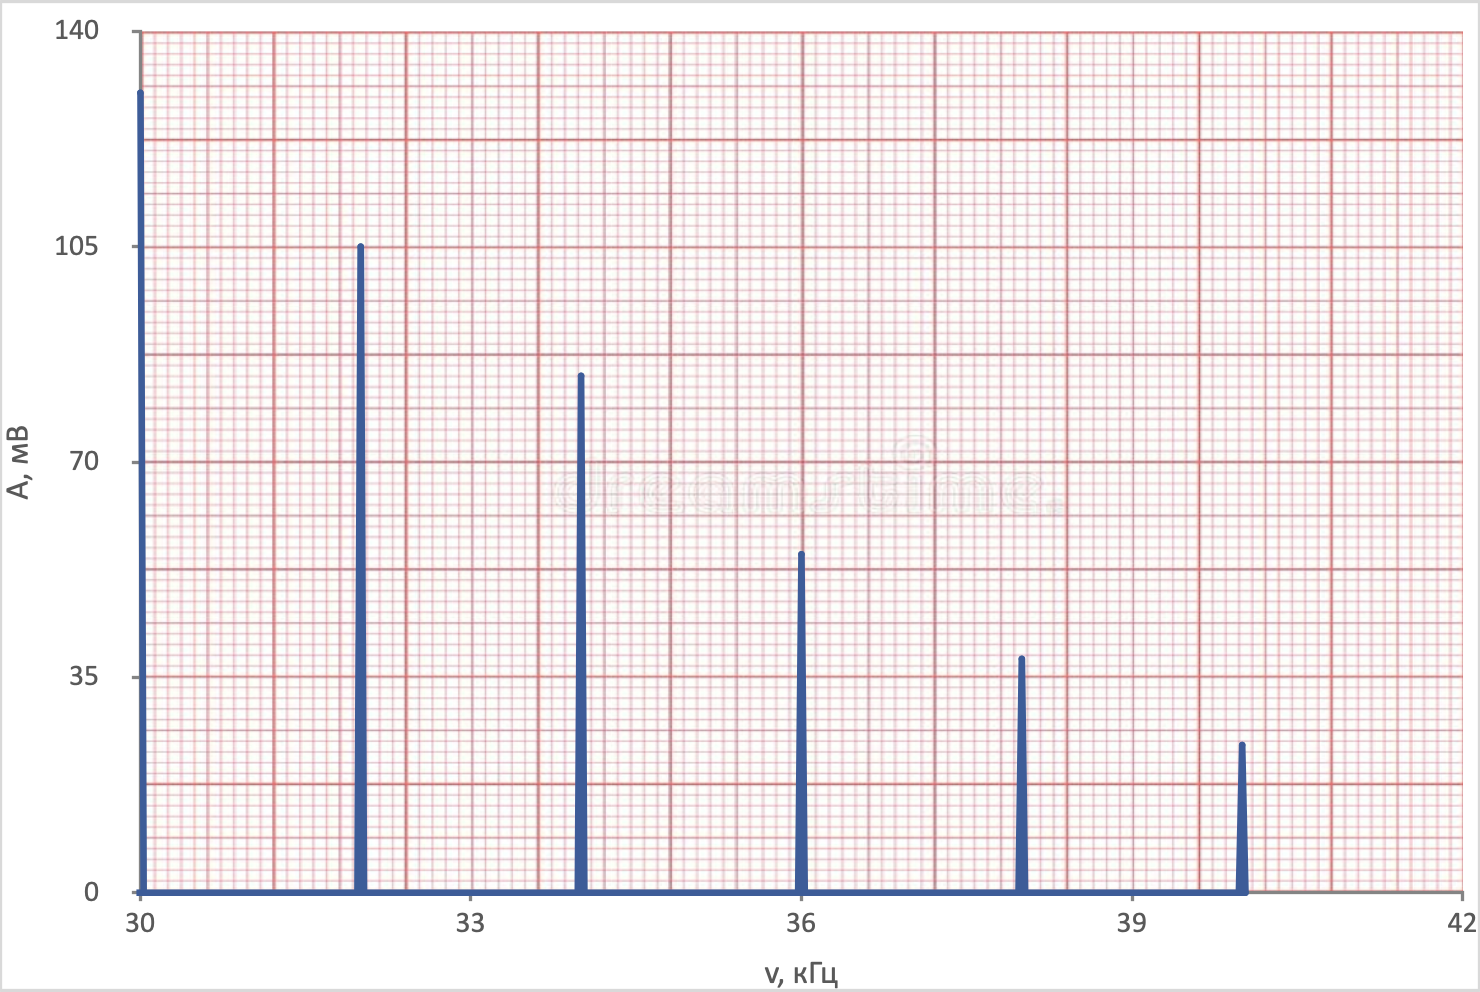
\includegraphics[width = 10 cm]{src/19_2.png}
	\caption{Спектр при $f_\text{повт}$ = 2 кГц}
	\label{fig:19_2}
\end{figure}

\subsection*{Исследование спектра гармонических сигналов, модулированных по амплитуде}

Будем менять двойную амплитуду сигнала канала $CH1$ от 0,2 до 2 В, измеряя для каждого значения боковую $A_\text{бок}$, основную боковую $A_\text{осн}$ (в спектре), максимальную $A_\text{макс}$ и минимальную $A_\text{мин}$ амплитуды сигналов. Измерения запишем в таблицу \ref{tab:26}.

\begin{table}[H]
    \caption{Измерения сигналов, модулированных по амплитуде}
    \begin{tabular}{ccccccc}
\toprule
$2A$, В & $A_\text{макс}$, мВ & $A_\text{мин}$, мВ & $A_\text{бок}$, мВ & $A_\text{осн}$, мВ & $m$ & $\frac{A_\text{бок}}{A_\text{осн}}$\\
\midrule
0,2 & 555 & 450 & 1,6 & 33,33 & 0,104 & 0,048 \\
0,4 & 602 & 402 & 3,2 & 32,99 & 0,199 & 0,097 \\
0,6 & 659 & 349 & 4,8 & 32,21 & 0,308 & 0,149 \\
0,8 & 716 & 294 & 6,4 & 32,49 & 0,418 & 0,197 \\
1,0 & 756 & 255 & 7,8 & 31,71 & 0,496 & 0,246 \\
1,2 & 806 & 202 & 9,4 & 32,53 & 0,599 & 0,289 \\
1,4 & 864 & 149 & 11,0& 32,26 & 0,706 & 0,341 \\
1,6 & 916 & 98  & 12,8& 32,32 & 0,807 & 0,396 \\
1,8 & 991 & 56  & 14,2& 32,27 & 0,893 & 0,440 \\
2,0 & 1000& 17	& 16,2& 32,40 & 0,967 & 0,500 \\	
\bottomrule
\end{tabular}

	\label{tab:26}
\end{table}

Построим график \ref{fig:26} отношения $\frac{A_\text{бок}}{A_\text{осн}}$ в зависимости от $m$ (рассчитывается по формуле \ref{eq:m}).
Коэффициент его наклона $k = (0,508 \pm 0,03) \;\;\;\; \varepsilon_k = 6 \%$ (рассчитан по МНК) отлично согласуется с теоретическим значением 0,5.

\begin{figure}[H]
	\centering
	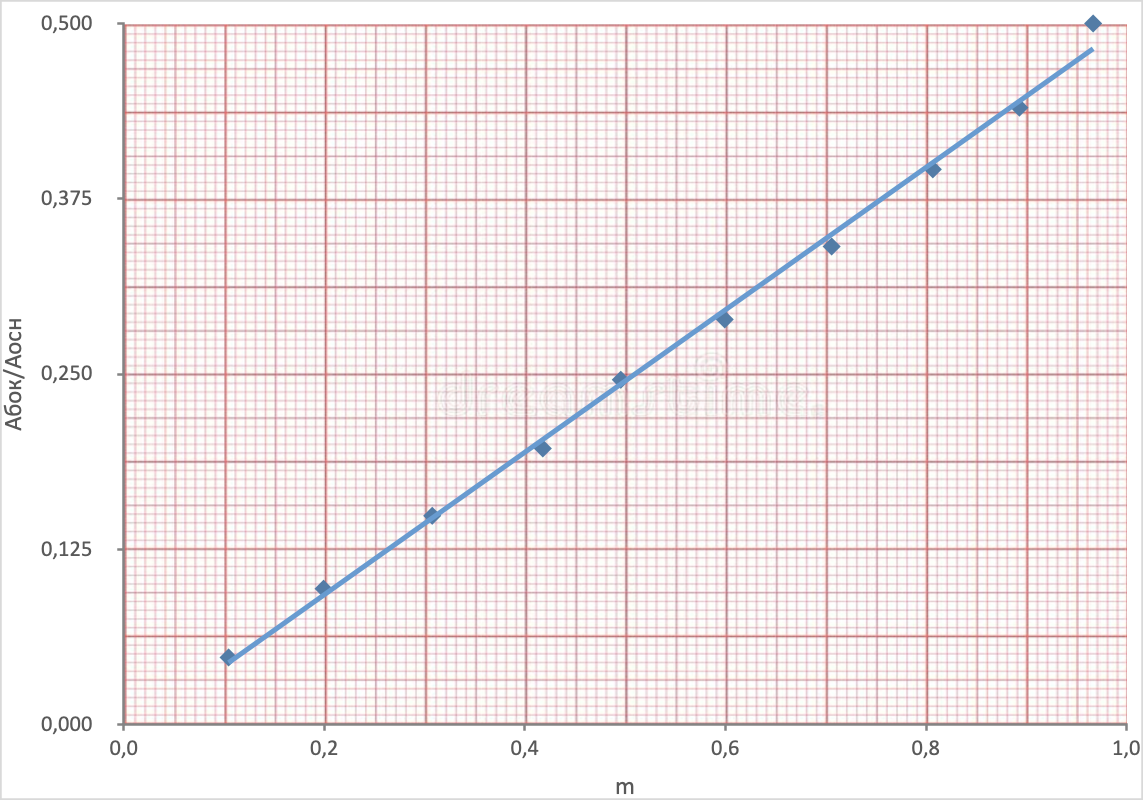
\includegraphics[width = 10 cm]{src/26.png}
	\caption{График зависимости $\frac{A_\text{бок}}{A_\text{осн}}(m)$}
	\label{fig:26}
\end{figure}


\subsection*{Исследование спектра гармонических сигналов, модулированных по частоте (дополнительное задание)}

Будем на генераторе изменять девитацию частоты $\Delta f_m$ от 100 до 1000 Гц, записывая амплитуду $A_0$ компоненты на основной частоте $\nu_0$ и амплитуды $A_{\pm1}$ на частотах $\nu_0 \pm F$ в таблицу \ref{tab:32}. При больших значениях $\Delta f_m$ запишем также $A_{\pm2}$ компонент на частотах $\nu_0 \pm 2F$.

\begin{table}[H]
    \caption{Спектр гармонического сигнала, модулированного по частоте}
    \begin{tabular}{ccccccc}
\toprule
$\Delta f_m$, Гц & $A_0$, мВ & $A_{\pm1}$, мВ & $A_{\pm2}$, мВ & $\beta$ & $\frac{A_{\pm1}}{A_0}(\beta)$\\
\midrule
100  & 308,1 & 15,38  &       & 0,1 & 0,050 \\
200  & 305,7 & 30,75  & 1,57  & 0,2 & 0,101 \\
300  & 302,6 & 44,86  & 3,45  & 0,3 & 0,148 \\
400  & 297,7 & 58,43  & 6,15  & 0,4 & 0,196 \\
500  & 289,7 & 72,57  & 9,23  & 0,5 & 0,251 \\
700  & 271,8 & 99,02  & 17,22 & 0,7 & 0,364 \\
1000 & 236,2 & 132,20 & 35,06 & 1,0 & 0,560 \\
\bottomrule
\end{tabular}

	\label{tab:32}
\end{table}

При частотах $\Delta f_m$ от 1 до 10 кГц спектр становится намного более сложным. Рассчитаем индекс модуляции $\beta$ для каждой $\Delta f_m$ и построим график \ref{fig:32} $\frac{A_{\pm1}}{A_0}(\beta)$. Проведём сглаживающую прямую. Её коэффициент наклона 0,4968 (рассчитан по МНК), что очень близко к теоретическому значению 0,5. 

\begin{figure}[H]
	\centering
	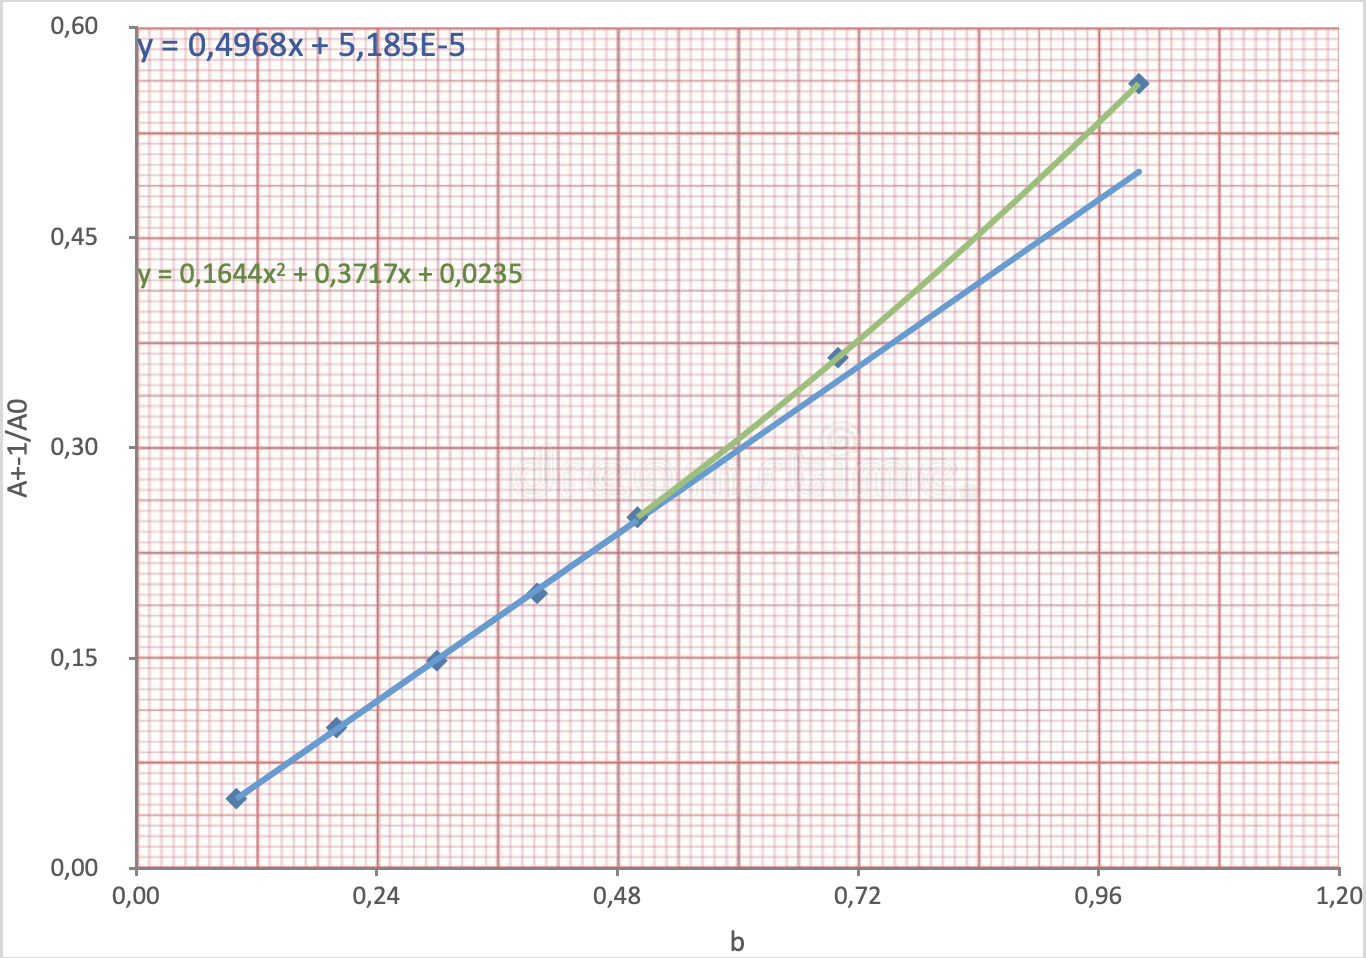
\includegraphics[width = 10 cm]{src/32.png}
	\caption{График зависимости $\frac{A_{\pm1}}{A_0}(\beta)$}
	\label{fig:32}
\end{figure}

Проэкстраполируем часть графика, плохо ложащуюся на проведенную прямую полиномом 2 степени. Тогда можно составить такое уравнение:

$$ 0,1644 \cdot \beta_\text{кр} ^ 2 + 0,3717 \cdot \beta_\text{кр} + 0,0235 - (0,4968 \cdot \beta_\text{кр} + 5,185E-5) = $$
$$ = 0,1 \cdot (0,4968 \cdot \beta_\text{кр} + 5,185E-5) \Rightarrow \beta_\text{кр} = 0,906 $$

Т. е. $\beta_\text{кр}$ = 0,906.

\newpage

\section*{Вывод}

Зависимость ширины спектра последовательности импульсов от длительности импульса полностью совпали с теоретическими рассчетами. По наклону графика \ref{fig:8} можно убедиться в соотношении неопределенностей $(\Delta \nu \tau \simeq 1)$.
 
Зависимость расстояния между ближайшими 
спектральными компонентами от частоты повторения цугов 
также подтвердилась. 

Коэффициенты, получаемые в результате зависимости отношения амплитуд спектральных линий сигнала, модулированного низкочастотными гармоническими колебаниями, от коэффициента модуляции сошлись с теоретически рассчитаными. 

В последней части работы был определён диапазон индексов модуляции, для которых амплитуда частотно-модулированного колебания практически не меняется.


\begin{thebibliography}{9}
	\bibitem{max} \emph{Лабораторный практикум по общей физике. В 3 томах. Том 2. Электричество и магнетизм: учебное пособие} под ред. А. В. Максимычева, М. Г. Никулина
\end{thebibliography}
\end{document}
